17. $y=\cfrac{|x-2|}{2-x}(x^2-2x)=\begin{cases}2x-x^2,\ x>2,\\ x^2-2x,\ x<2.\end{cases}$
$$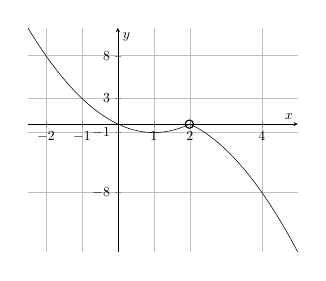
\begin{tikzpicture}[scale=0.5]
\begin{axis}[
    axis lines = middle,
    grid=major,
    legend pos={south west},
    xlabel = {$x$},
    %xlabel style={below right},
    ylabel = {$y$},
    xtick={-2, -1,1, 2,4},
    ytick={8,3,-1,-8},
                  ]
	\addplot[domain=-2.5:2, samples=100, color=black] {x*x-2*x};
    \addplot[domain=2:5, samples=100, color=black] {-x*x+2*x};
	%\addlegendentry{$\text{Рис. 1}$};
\end{axis}
\draw (4.1,3.25) circle (3pt);
\end{tikzpicture}$$
